\subsection{Luthfi Muhammad Nabil/1174035}
\subsubsection{Pemahaman Teori}
\begin{enumerate}
	\item Fungsi adalah sintaks yang terdiri dari nama fungsi, parameter input variabel, dan variabel kembali. Pada python, nama fungsi diawali dengan def dan pada sintaks paling akhir (setelah parameter) adalah titik dua. Aturan penamaan dari fungsi sama dengan penamaan sebuah variabel yang salah satunya yaitu case sensitive. Untuk penulisan parameter tidak harus memasukan inputan dan batas untuk penulisan variabel pada parameter tidak memiliki batas atau bisa lebih dari satu dengan pemisah tanda koma. Nilai yang dapat dikembalikan oleh fungsi dapat berupa variabel yang mau dikembalikan. Berikut contoh dari koding fungsi : 
	\lstinputlisting[firstline=1, lastline=4]{src/chapter3/chap3_1174035_teori.py}
	\item Paket merupakan sebuah file yang berisikan fungsi - fungsi yang dapat dipakai. Untuk pemanggilan fungsi diperlukan keyword import untuk memanggil paket tersebut. berikut contoh pemakaian dari paket : 
	\lstinputlisting[firstline=6, lastline=8]{src/chapter3/chap3_1174035_teori.py}
	\item Class merupakan cetak biru dari sebuah objek yang dibuat. Objek merupakan instansi dari sebuah class. Atribut merupakan variabel atau yang menampung nilai pada sebuah objek. Fungsi adalah sebuah pembungkus kumpulan instruksi pada sebuah program. Berikut contohnya : 
	\lstinputlisting[firstline=10, lastline=24]{src/chapter3/chap3_1174035_teori.py}
	\item Pemanggilan sebuah kelas diawali dari sebuah paket dipanggil terlebih dahulu, lalu kelas akan disimpan ke variabel untuk diinisiasi sebagai objek. Berikut contoh pemanggilan dari kelas : 
	\lstinputlisting[firstline=26, lastline=29]{src/chapter3/chap3_1174035_teori.py}
	\item Pemakaian from kalkulator merupakan sebuah inisiasi untuk memanggil fungsi penambahan dari paket kalkulator yang dipanggil agar fungsi penambahandapat digunakan langsung tanpa menulis nama file dari paket yaitu kalkulator. Berikut Contohnya : 
	\lstinputlisting[firstline=31, lastline=34]{src/chapter3/chap3_1174035_teori.py}
	\item Pemakaian paket fungsi memanggil fungsi dari paket lain dan memanggil paket tersebut dengan tambahan nama asal paket dari fungsi yang akan dipanggil. Berikut pemakaiannya : 
	\lstinputlisting[firstline=36, lastline=39]{src/chapter3/chap3_1174035_teori.py}
	\item Pemakaian paket kelas sama halnya dengan fungsi hanya saja untuk paket kelas diinisiasikan terlebih dahulu lalu nilai variabel akan dikirim ke constructor dari class tersebut. Pada saat memanggil fungsi tidak perlu menggunakan inputan parameter karena nilai yang dikirim sudah disimpan pada constructor di class yang dipanggil. Berikut Contohnya : 
	\lstinputlisting[firstline=41, lastline=46]{src/chapter3/chap3_1174035_teori.py}
\end{enumerate}
\subsection{Ketrampilan Pemrograman}
\begin{enumerate}
	\item Membuat fungsi dengan inputan variabel NPM, dan melakukan print luaran huruf yang dirangkai dari tanda bintang, paga,r, plus dari NPM kita. Untuk NPM mod 3=0 memakai bintang, NPM mod 3=1 memakai pagar, NPM mod 3 = 2 memakai tanda plus. Kodingnya : 
	\lstinputlisting{src/chapter3/chap3_1174035_1.py}
	\begin{figure}[!htbp]
        \centering
        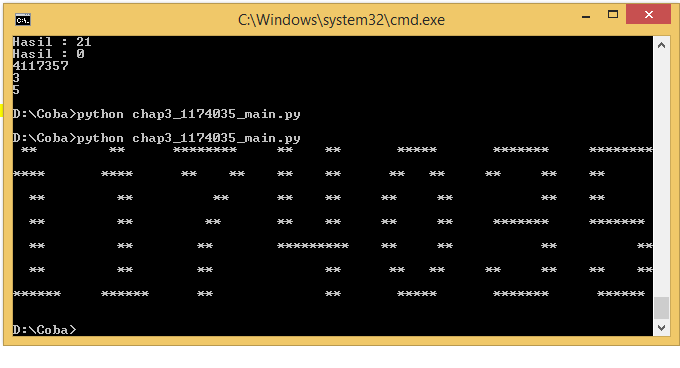
\includegraphics[height=7cm, width=10cm]{figures/chapter3/1174035_1.png}
        \caption{Screenshot No 1}
        \label{1174035_1}
	\end{figure}
	\item Membuat fungsi dengan inputan variabel NPM, dan lakukan perulangan untuk mengeluarkan print output sebanyak dua dijit belakang NPM. Contoh NPM : 1174035 maka akan ada output sebanyak 35 kali dengan tulisan 'Hallo, 1174035 apa kabar?' Kodingnya : 
	\lstinputlisting{src/chapter3/chap3_1174035_2.py}
	\begin{figure}[!htbp]
        \centering
        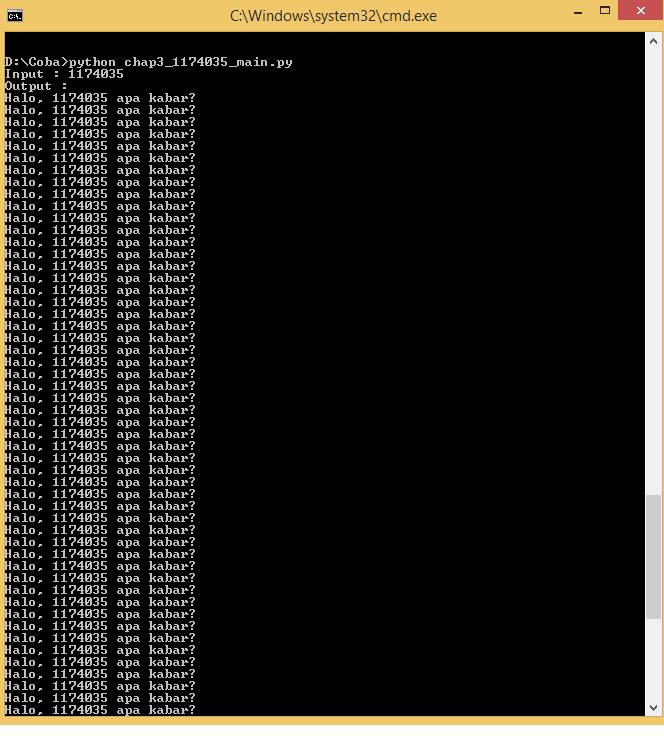
\includegraphics[height=7cm, width=10cm]{figures/chapter3/1174035_2.png}
        \caption{Screenshot No 2}
        \label{1174035_2}
	\end{figure}
	\item Membuat fungsi dengan inputan variabel NPM, dan melakukan print luaran output dengan perulangan berupa tiga karakter belakang dari NPM dijumlahkan. Lalu jumah perulangan tersebut adalah total dari tiga karakter belakang NPM dijumlahkan. Kodingnya : 
	\lstinputlisting{src/chapter3/chap3_1174035_3.py}
	\begin{figure}[!htbp]
        \centering
        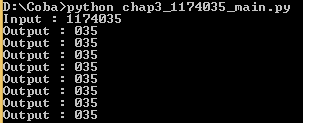
\includegraphics[height=7cm, width=10cm]{figures/chapter3/1174035_3.png}
        \caption{Screenshot No 3}
        \label{1174035_3}
	\end{figure}
	\item Membuat fungsi dengan inputan variabel NPM, dan melakukan print hello world dan digit ketiga dari belakang dari NPM. contoh : NPM : 0, Output : Halo, 0 apa kabar? .Kodingnya : 
	\lstinputlisting{src/chapter3/chap3_1174035_4.py}
	\begin{figure}[!htbp]
        \centering
        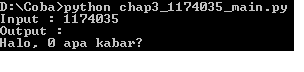
\includegraphics[height=3cm, width=8cm]{figures/chapter3/1174035_4.png}
        \caption{Screenshot No 4}
        \label{1174035_4}
	\end{figure}
	\item Membuat fungsi dengan inputan variabel NPM, dan menampilkan semua angka dari NPM tersebut secara berurutan kebawah. Kodingnya : 
	\lstinputlisting{src/chapter3/chap3_1174035_5.py}
	\begin{figure}[!htbp]
        \centering
        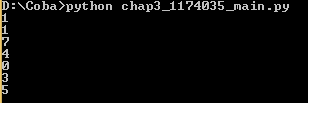
\includegraphics[height=5cm, width=10cm]{figures/chapter3/1174035_5.png}
        \caption{Screenshot No 5}
        \label{1174035_5}
	\end{figure}
	\item Membuat fungsi dengan inputan variabel NPM, didalamnya melakukan penjumlahan dari seluruh dijit NPM tersebut. menggunakan perulangan atau kondisi. Kodingnya : 
	\lstinputlisting{src/chapter3/chap3_1174035_6.py}
	\begin{figure}[!htbp]
        \centering
        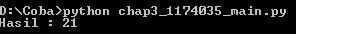
\includegraphics[height=5cm, width=10cm]{figures/chapter3/1174035_6.png}
        \caption{Screenshot No 6}
        \label{1174035_6}
	\end{figure}
	\item Membuat fungsi dengan inputan variabel NPM, didalamnya melakukan perkalian dari seluruh dijit NPM tersebut. menggunakan perulangan atau kondisi. Kodingnya : 
	\lstinputlisting{src/chapter3/chap3_1174035_7.py}
	\begin{figure}[!htbp]
        \centering
        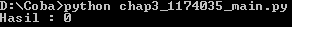
\includegraphics[height=4cm, width=10cm]{figures/chapter3/1174035_7.png}
        \caption{Screenshot No 7}
        \label{1174035_7}
	\end{figure}
	\item Membuat fungsi dengan inputan variabel NPM, lalu lakukan print seluruh angka genap dari setiap angka di NPM. Kodingnya : 
	\lstinputlisting{src/chapter3/chap3_1174035_8.py}
	\begin{figure}[!htbp]
        \centering
        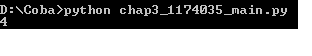
\includegraphics[height=4cm, width=10cm]{figures/chapter3/1174035_8.png}
        \caption{Screenshot No 8}
        \label{1174035_8}
	\end{figure}
	\item Membuat fungsi dengan inputan variabel NPM, lalu lakukan print seluruh angka ganjil dari setiap angka di NPM. Kodingnya : 
	\lstinputlisting{src/chapter3/chap3_1174035_9.py}
	\begin{figure}[!htbp]
        \centering
        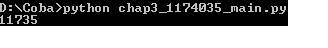
\includegraphics[height=4cm, width=10cm]{figures/chapter3/1174035_9.png}
        \caption{Screenshot No 9}
        \label{1174035_9}
	\end{figure}
	\item Membuat fungsi dengan inputan variabel NPM, lalu lakukan print seluruh angka prima dari setiap angka di NPM. Kodingnya : 
	\lstinputlisting{src/chapter3/chap3_1174035_10.py}
	\begin{figure}[!htbp]
        \centering
        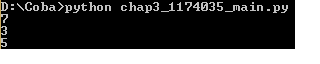
\includegraphics[height=5cm, width=10cm]{figures/chapter3/1174035_10.png}
        \caption{Screenshot No 10}
        \label{1174035_10}
	\end{figure}
	\item Membuat Satu File library bernama 3lib.py yang berisi semua fungsi - fungsi dari setiap nomor pada soal praktek. Kodingnya : 	
	\lstinputlisting{src/chapter3/chap3_1174035_3lib.py}
	\lstinputlisting[firstline=1, lastline=15]{src/chapter3/chap3_1174035_main.py}
	
	\begin{figure}[!htbp]
        \centering
        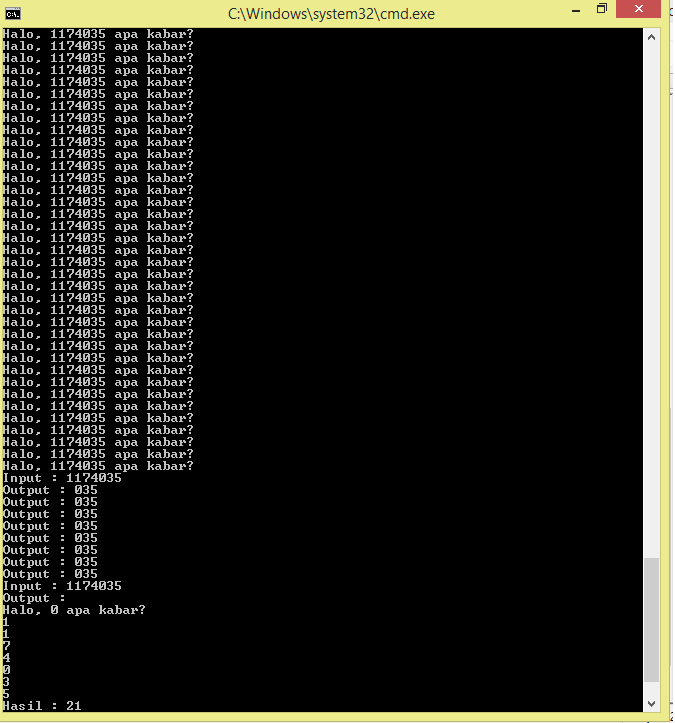
\includegraphics[height=10cm, width=8cm]{figures/chapter3/1174035_3lib.png}
        \caption{Screenshot No 11}
        \label{1174035_3lib}
	\end{figure}
	
	\item Membuat Satu File library bernama kelas3lib.py yang berisi kelas yang isinya semua fungsi - fungsi dari setiap nomor yang telah dimodifikasi untuk menyesuaikan dengan kelas. Kodingnya : 	
	\lstinputlisting{src/chapter3/chap3_1174035_kelas3lib.py}
	\lstinputlisting[firstline=16, lastline=29]{src/chapter3/chap3_1174035_main.py}
	
	\begin{figure}[!htbp]
        \centering
        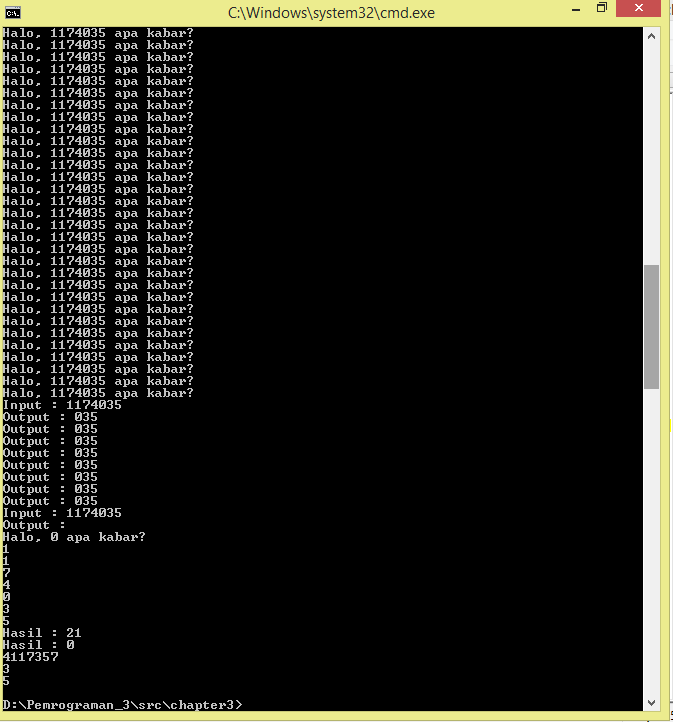
\includegraphics[height=10cm, width=8cm]{figures/chapter3/1174035_kelas3lib.png}
        \caption{Screenshot No 12}
        \label{1174035_kelas3lib}
	\end{figure}
	
	
\end{enumerate}

\subsubsection{Error}
\begin{enumerate}
	\item Tuliskan error yang terjadi saat mengerjakan section ini. Mendapat error yaitu salah konversi. Untuk menghandle error tersebut dapat menggunakan try catch :
	\lstinputlisting{src/chapter3/chap3_1174035_error.py}
	\lstinputlisting[firstline=32, lastline=36]{src/chapter3/chap3_1174035_main.py}
	\begin{figure}[!htbp]
        \centering
        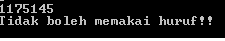
\includegraphics[height=3cm, width=8cm]{figures/chapter3/1174035_error.png}
        \caption{Screenshot No 13}
        \label{1174035_error}
	\end{figure}
	\item Plagiarisme
	\begin{figure}[!htbp]
        \centering
        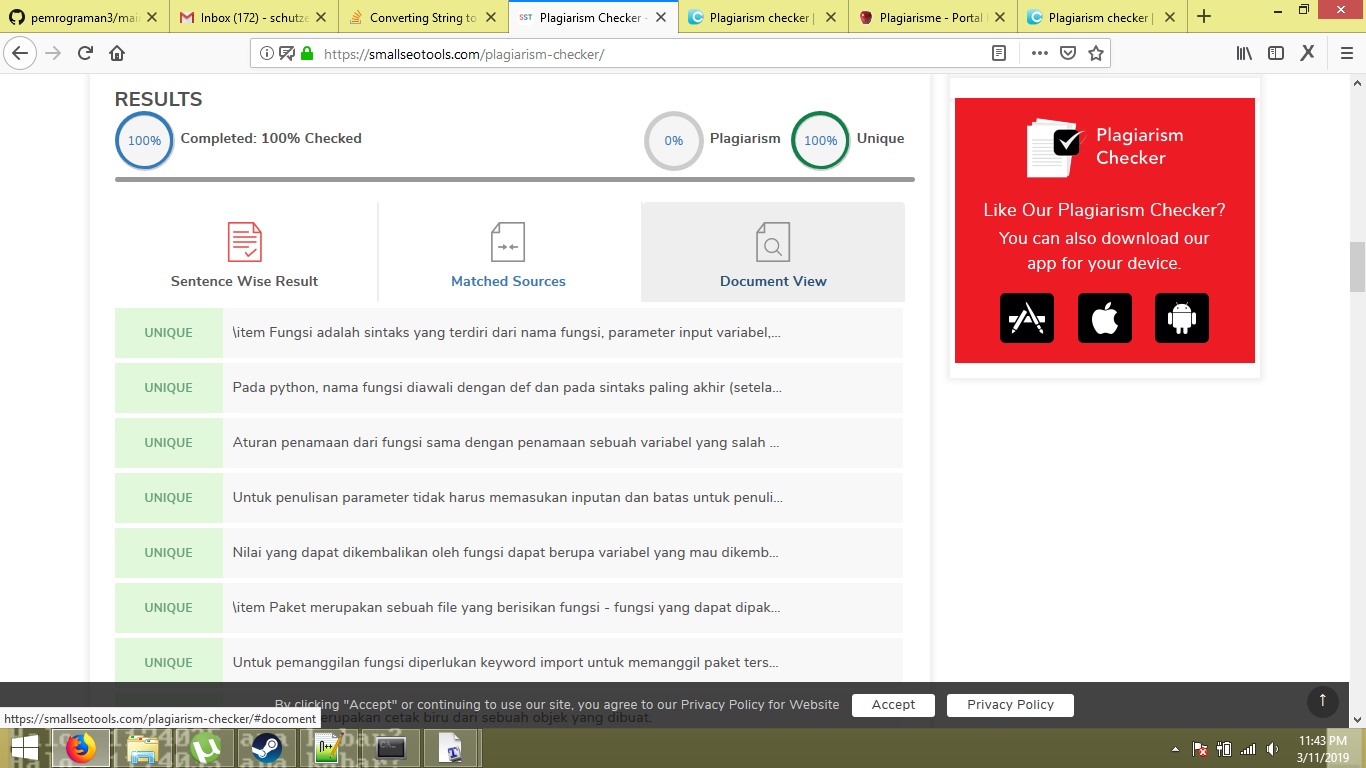
\includegraphics[height=7cm, width=9cm]{figures/chapter3/1174035_plagiarisme.png}
        \caption{Plagiarisme}
        \label{1174035_plagiarisme}
	\end{figure}
\end{enumerate}